% This is samplepaper.tex, a sample chapter demonstrating the
% LLNCS macro package for Springer Computer Science proceedings;
% Version 2.21 of 2022/01/12
%
\documentclass[runningheads]{llncs}
%
\usepackage[T1]{fontenc}
% T1 fonts will be used to generate the final print and online PDFs,
% so please use T1 fonts in your manuscript whenever possible.
% Other font encondings may result in incorrect characters.
%
\usepackage{graphicx}
\usepackage{amsmath,amssymb}
\usepackage{subcaption}
\usepackage{float}
\usepackage[hidelinks]{hyperref}
\usepackage{xcolor}  % temporary import for editing

% Used for displaying a sample figure. If possible, figure files should
% be included in EPS format.
%
% If you use the hyperref package, please uncomment the following two lines
% to display URLs in blue roman font according to Springer's eBook style:
%\usepackage{color}
%\renewcommand\UrlFont{\color{blue}\rmfamily}
%\urlstyle{rm}
%
\begin{document}
%
\title{State-Dependent Lagrange Multipliers for State-Wise Safety in Constrained Reinforcement Learning}
%
\titlerunning{State-Dependent Lagrange Multiplier for State-Wise Safety in CRL}
% If the paper title is too long for the running head, you can set
% an abbreviated paper title here
%
\author{Minseok Seo \and Kyunghwan Choi}
%
\authorrunning{M. Seo and K. Choi}
% First names are abbreviated in the running head.
% If there are more than two authors, 'et al.' is used.
%
\institute{Cho Chun Shik Graduate School of Mobility, KAIST 
\email{\{seominseok,kh.choi\}@kaist.ac.kr} \\
\url{https://kaist-mic-lab.github.io}}
%
\maketitle              % typeset the header of the contribution
%

\begin{abstract}
    Despite the remarkable success of deep reinforcement learning (deep RL) across various domains, its deployment in the real world remains limited due to safety concerns.
    To address this challenge, constrained reinforcement learning (constrained RL) has been extensively studied as an approach for learning safe policies while maintaining performance.
    However, since constrained RL enforces constraints in the form of cumulative costs, it cannot guarantee state-wise safety.
    In this paper, we extend the Lagrangian based approach, a representative method in constrained RL, by introducing state-dependent Lagrange multipliers so that the policy is trained to account for state-wise safety.
    Our results show that the proposed method enables more fine-grained specification of the constraints and allows the policy to satisfy them more effectively by employing state-dependent Lagrange multipliers instead of a single scalar multiplier.
\end{abstract}
\section{INTRODUCTION}

Reinforcement learning (RL) learns policy that maximize rewards through trial and error.
This way of learning the desired behaviors may seem simple and straightforward, but it is highly effective.
Over the past few years, RL has demonstrated impressive achievements in diverse applications ... \cite{silver2017mastering} \cite{andrychowicz2020learning} \cite{ouyang2022training}.
Nevertheless, deploying RL in physical real-world environments remains a major challenge.
To deploy RL-trained agents in real-world environments, two requirements must be satisfied:
\textcolor{red}{First}, the ability to successfully accomplish the given tasks, and second, the safety and reliability of the learned agent.
In standard RL, such requirements are learned exclusively from reward signals, thereby necessitating careful reward engineering.
However, even with carefully designed rewards and successful training in simulation, the learned policy may fail when tasks change or when transferring to real-world environments, due to issues such as reward hacking or lack of generalization \cite{amodei2016concrete}.
To address these issues, constrained reinforcement learning (constrained RL) has recently been widely studied.

Constrained RL is a method that learns policy maximizing rewards while satisfying constraints, thus enabling agents to behave safely while successfully performing tasks.
A common formulation of constrained RL specifies constraints at the trajectory level \cite{brunke2022safe}.
As a result, since the constraints are specified over entire trajectory, violations occurring at individual timesteps cannot be directly \textcolor{red}{constrained/restricted.}
For example, even if a constraint is defined to limit the number of lane departures during the entire trip of an autonomous vehicle, a single deviation from the lane that results in a collision with another vehicle can lead to a catastrophic failure.
This illustrates that trajectory-level constraints regulate only the outcome of a task \textcolor{red}{but are limited in controlling the risky process itself.}
Therefore, in this paper, we propose an approach that considers state-wise constraints.
Specifically, we extend the Lagrangian-based approach, a representative method in constrained RL, by introducing state-wise Lagrange multipliers so that the policy is encouraged to take safe actions at every timestep.
\section{Related Work}
\section{Methodology}

%%%%%%%%%%%%%%%%%%%%%%%%%%%%%%%%
% Preliminaries
%%%%%%%%%%%%%%%%%%%%%%%%%%%%%%%%

\subsection{Preliminaries}

\subsubsection{Problem Formulations}

\paragraph{\textbf{Markov Decision Processes}}

% ! 그냥 In RL이라고 써도 되는건지?
In RL, problems are typically formulated as a Markov decision process (MDP) \cite{sutton1998reinforcement}.
An MDP is defined as a tuple $\langle S, A, P, R, \gamma \rangle$, where $S$ and $A$ denote the state and action spaces, $P$ is the transition probability, $R$ is the reward function, and $\gamma \in [0, 1)$ is the discount factor.
The objective of RL is to find an optimal policy $\pi^*$ that maximizes the cumulative reward defined as:
\begin{equation} \label{eq:mdp_optimization_problem}
    \begin{aligned}
        J_R(\pi) &= \mathbb{E}_{\tau \sim \pi}\!\left[\sum^\infty_{t = 0} \gamma^t R(s_t, a_t)\right] \\
        \pi^* &= \arg \max J_R(\pi)
    \end{aligned}
\end{equation}
Here, $\tau = (s_0, a_0, s_1, a_1, \ldots)$ denotes a trajectory \textcolor{red}{under} policy $\pi$.

\paragraph{\textbf{Constrained Markov Decision Processes}}

In contrast, constrained RL is typically formulated as a constrained Markov decision process (CMDP) \cite{altman2021constrained}.
\textcolor{red}{A CMDP extends an MDP by introducing cost functions $C_1, \ldots, C_m$ (separate from the reward function) and their corresponding limits $d_1, \ldots, d_m$.}
Formally, a CMDP is defined as a tuple $\langle S, A, P, R, C, d, \gamma \rangle$.
In a CMDP, the set of feasible policies $\Pi_C$ is defined as:
\begin{equation} \label{eq:feasible_policy_set_cmdp}
    \begin{aligned}
        \Pi_C = \{ \pi \in \Pi: \forall i \in \{1, \ldots, m\}, \; J_{C_i}(\pi) \leq d_i \}.
    \end{aligned}
\end{equation}
Specifically, the constraint function for constraint $i$ is defined as the expected cumulative discounted cost:
\begin{equation} \label{eq:cost_return}
    J_{C_i}(\pi) = \mathbb{E}_{\tau \sim \pi}\!\left[\sum^\infty_{t = 0} \gamma^t C_i(s_t, a_t)\right], 
    \quad \forall i \in \{1, \ldots, m\}.
\end{equation}
In standard RL, the objective is an unconstrained policy optimization problem that aims to find a policy maximizing the expected return, as defined in Eq.~\eqref{eq:mdp_optimization_problem}, \textcolor{red}{whereas constrained RL seeks to maximize the expected return subject to the cost constraints defined in Eq.~\eqref{eq:cost_return}.}
\begin{equation} \label{eq:cmdp_optimization_problem}
    \pi^* = \arg\max_\pi J_R(\pi) \; \text{s. t.} \; \pi \in \Pi_C.
\end{equation}


\paragraph{\textbf{State-wise Constrained Markov Decision Process}}

The CMDP framework can be extended to \textcolor{red}{incorporate cost-based constraints of different forms.}
One such extension is the state-wise constrained Markov decision process (SCMDP) \cite{zhao2023state}, which \textcolor{red}{enforces constraints that bound the expected cost at each state by a specified threshold.}
In a SCMDP, the set of feasible policies $\Pi_{SC}$ is defined as:
\begin{equation} \label{eq:feasible_policy_set_scmdp}
    \begin{aligned}    
        \Pi_{SC} = \{ \pi \in \Pi: &\;\forall i \in \{1, \ldots, m\}, \; J_{{SC}_i}(\pi) \leq w_i \}.
    \end{aligned}
\end{equation}
In this definition, the state-wise constraint represents the expected cost incurred at each state:
\begin{equation} \label{eq:statewise_cost_return}
    J_{{SC}_i}(\pi) = \mathbb{E}_{(s_t, a_t, s_{t + 1}) \sim \tau, \, \tau \sim \pi} \big[ C_i(s_t, a_t, s_{t + 1}) \big], 
    \quad \forall i \in \{1, \ldots, m\}.
\end{equation}
Consequently, similar to CMDP, the optimization problem in SCMDP can be formulated as:
\begin{equation} \label{eq:scmdp_optimization_problem}
    \pi^* = \arg\max_\pi J_R(\pi) \; \text{s.t.} \; \pi \in \Pi_{SC}.
\end{equation}  % refrence: https://arxiv.org/pdf/2306.12594
\textcolor{red}{In a CMDP, constraints are imposed on the cumulative cost, whereas an SCMDP enforces constraints on the expected cost at each state.}
\textcolor{red}{This enables safety guarantees at the state level, as illustrated in Fig.~\ref{fig:constrained_rl_vs_statewise_constrained_rl}.}
% TODO: cost 계산만 다르게 할거면 그림은 통일
% TODO: 그림 quality가 낮음
% TODO: caption의 설명을 어디서 할건지? 지금까지 설명한 내용으로 충분하지 않은가요?
\begin{figure}[H]
    \centering

    % (a) Constrained RL
    \begin{subfigure}{0.46\textwidth}
        \centering
        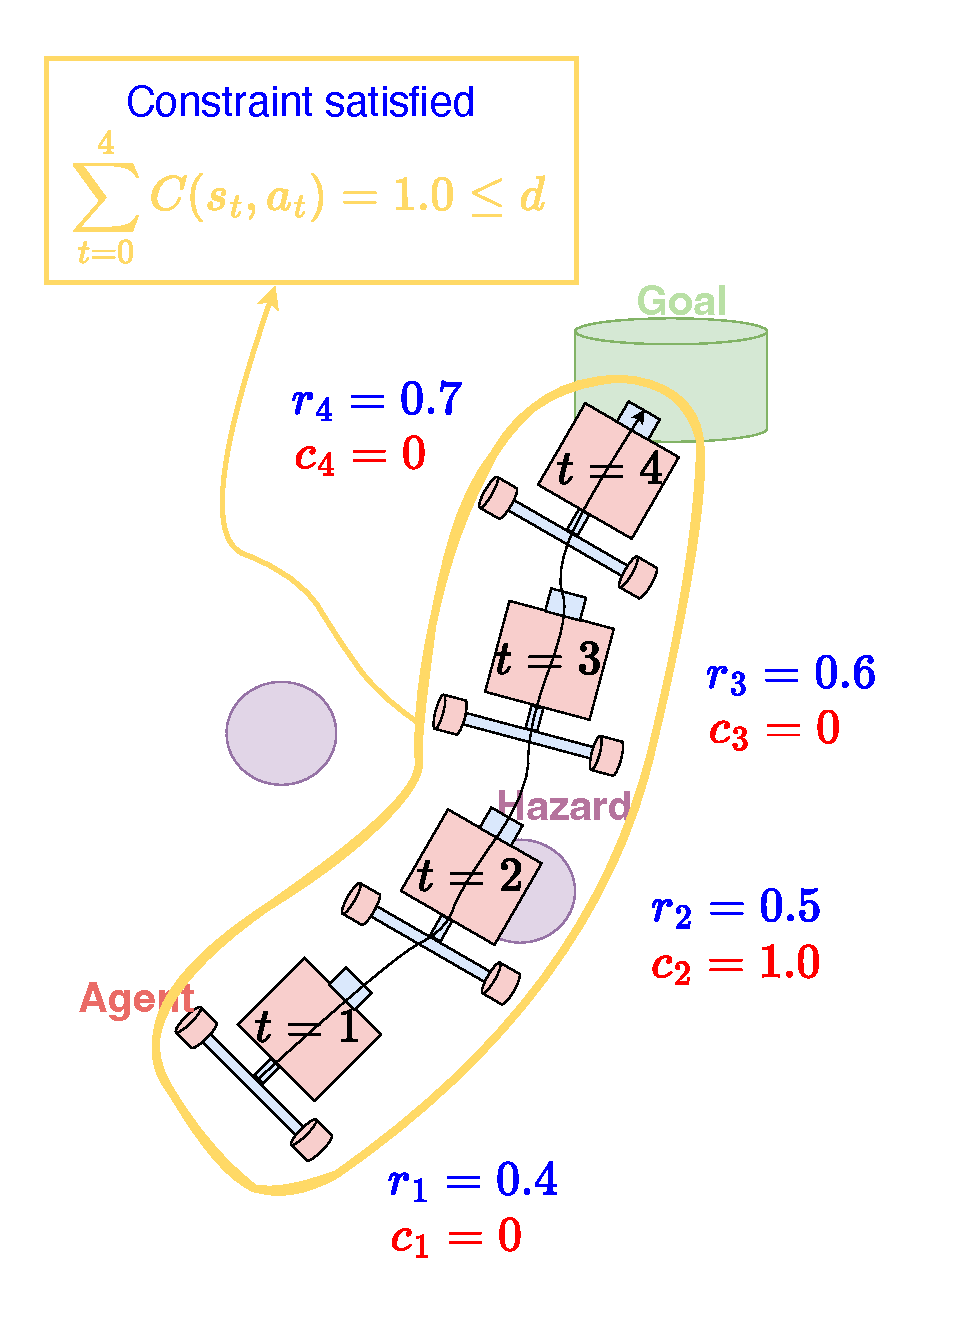
\includegraphics[width=\linewidth]{figure/constrained-rl.pdf}
        \caption{Constrained RL}
    \end{subfigure}
    \hfill
    % (b) State-wise constrained RL
    \begin{subfigure}{0.48\textwidth}
        \centering
        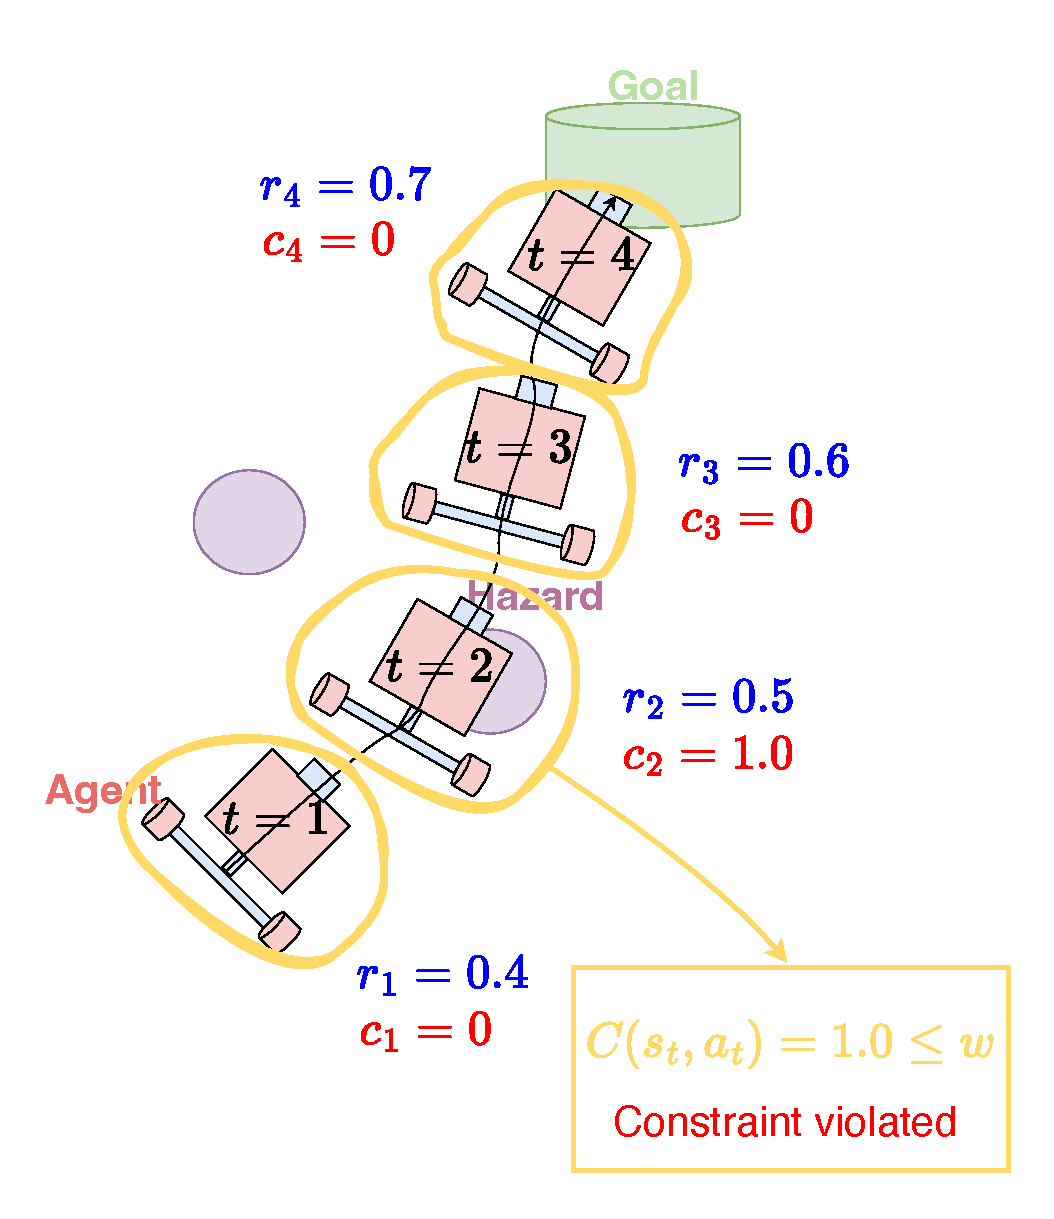
\includegraphics[width=\linewidth]{figure/statewise-constrained-rl.pdf}
        \caption{State-wise constrained RL}
    \end{subfigure}
    \caption{Comparison of constrained RL and state-wise constrained RL.
            In constrained RL, a policy is feasible if the cumulative cost is below the limit.
            In state-wise constrained RL, a policy is feasible if the cost at every state is below the limit.}
    \label{fig:constrained_rl_vs_statewise_constrained_rl}
\end{figure}



\subsubsection{Lagrangian Relaxation for Constrained Policy Optimization} \label{subsubsec:lagrangian_relaxation}

A common approach to solve constrained optimization problems is \textcolor{red}{to use the Lagrangian relaxation method.}
In this approach, the constrained optimization problem \eqref{eq:cmdp_optimization_problem} is reformulated as an unconstrained optimization problem by introducing Lagrange multiplier $\lambda \geq 0$ that penalizes constraint violations.
The resulting Lagrangian can be written as:
\begin{equation}
    L(\theta, \lambda) = J_R(\pi_\theta) - \lambda^\top (J_C(\pi_\theta) - d),
\end{equation}
where $\theta$ denotes the parameter of the policy.
The objective is then to find a saddle point $(\theta^*, \lambda^*)$ that satisfies:
\begin{equation}
    L(\theta^*, \lambda) \geq L(\theta^*, \lambda^*) \geq L(\theta, \lambda^*).
\end{equation}
Since finding a global saddle point is \textcolor{red}{typically} intractable, in practice, one seeks a locally optimal solution by iteratively updating the policy parameters and the Lagrange multipliers.
A common approach is to apply gradient-based updates of the form
\begin{align}
    \theta_{n+1} &= \theta_n + \eta_\theta \nabla_\theta \Big(J_R(\pi_\theta) - \lambda_n^\top J_C(\pi_\theta)\Big), \\
    \lambda_{n+1} &= \Big[ \lambda_n + \eta_\lambda \big( J_C(\pi_\theta) - d \big) \Big]_+,
\end{align}
where $\eta_\theta, \eta_\lambda > 0$ are step sizes, and $[\cdot]_+$ denotes the projection onto the nonnegative reals to ensure $\lambda \geq 0$.

%%%%%%%%%%%%%%%%%%%%%%%%%%%%%%%%
% PPO Lagrangian
%%%%%%%%%%%%%%%%%%%%%%%%%%%%%%%%

\subsection{Formulations of PPO under MDP and CMDP}

\paragraph{\textbf{PPO}}

Among policy gradient methods, PPO is one of the most widely used algorithms, proposed to solve the optimization problem in Eq.~\eqref{eq:mdp_optimization_problem}.
To improve stability, PPO introduces a clipping mechanism that prevents large policy updates.
The objective function of PPO is defined as:
\begin{equation} \label{eq:ppo_objective}
    J^{\text{PPO}}(\theta) = \mathbb{E}_{\pi_{\theta_\text{old}}} \left[ \min \left( r(\theta) A^{\pi_{\theta_\text{old}}}_R (s, a), \text{clip}(r(\theta), 1 - \epsilon, 1 + \epsilon) A^{\pi_{\theta_\text{old}}}_R (s, a) \right) \right]
\end{equation}
where $r(\theta) = \frac{\pi_\theta(a|s)}{\pi_{\theta_\text{old}}(a|s)}$ denotes the probability ratio between the current and the old policies, and $A^{\pi_{\theta_\text{old}}}_R (s, a) = Q^{\pi_{\theta_\text{old}}}_R (s, a) - V^{\pi_{\theta_\text{old}}}_R (s)$ represents the \textit{reward advantage function} under the old policy.

\paragraph{\textbf{PPO Lagrangian}}

PPO Lagrangian extends PPO to the constrained RL setting, allowing the algorithm to handle explicit constraints.
The original PPO algorithm enhances stability by limiting policy updates through clipping, as defined in Eq.~\eqref{eq:ppo_objective}, but it does not \textcolor{red}{explicitly account for constraints.}
To address constraints defined in terms of the cumulative cost in Eq.~\eqref{eq:cost_return}, PPO Lagrangian applies the Lagrangian relaxation technique, as discussed in Section~\ref{subsubsec:lagrangian_relaxation}, thereby converting the constrained optimization problem in Eq.~\eqref{eq:cmdp_optimization_problem} into an unconstrained one.
\textcolor{red}{For simplicity, we consider a single-constraint case throughout this paper, although the original formulation supports multiple constraints.}
\begin{equation} \label{eq:ppo_lagrangian_objective}
    \begin{aligned} J^{\text{PPO-Lag}}(\theta)
        = \mathbb{E}_{\pi_{\theta_\text{old}}} \Big[ &\min \big( r(\theta) A^{\pi_{\theta_\text{old}}}_R (s, a), \text{clip}(r(\theta), 1 - \epsilon, 1 + \epsilon) A^{\pi_{\theta_\text{old}}}_R (s, a) \big)
        \\ &- \lambda r(\theta) A^{\pi_{\theta_\text{old}}}_C (s, a) \Big]
    \end{aligned}
\end{equation}
where $\lambda \geq 0$ is the Lagrange multiplier that imposes a penalty on constraint violations, and \textcolor{red}{$A^{\pi_{\theta_\text{old}}}_C(s, a) = Q^{\pi_{\theta_\text{old}}}_C(s, a) - V^{\pi_{\theta_\text{old}}}_C(s)$ denotes the \textit{cost advantage function} under the old policy.}


%%%%%%%%%%%%%%%%%%%%%%%%%%%%%%%%
% Methodology
%%%%%%%%%%%%%%%%%%%%%%%%%%%%%%%%

\subsection{Proposed Method}


% TODO: 이 figure를 쓸거면 본문에서 언급해야 함
% TODO: figure quality가 낮음

\begin{figure}[h]
    \centering

    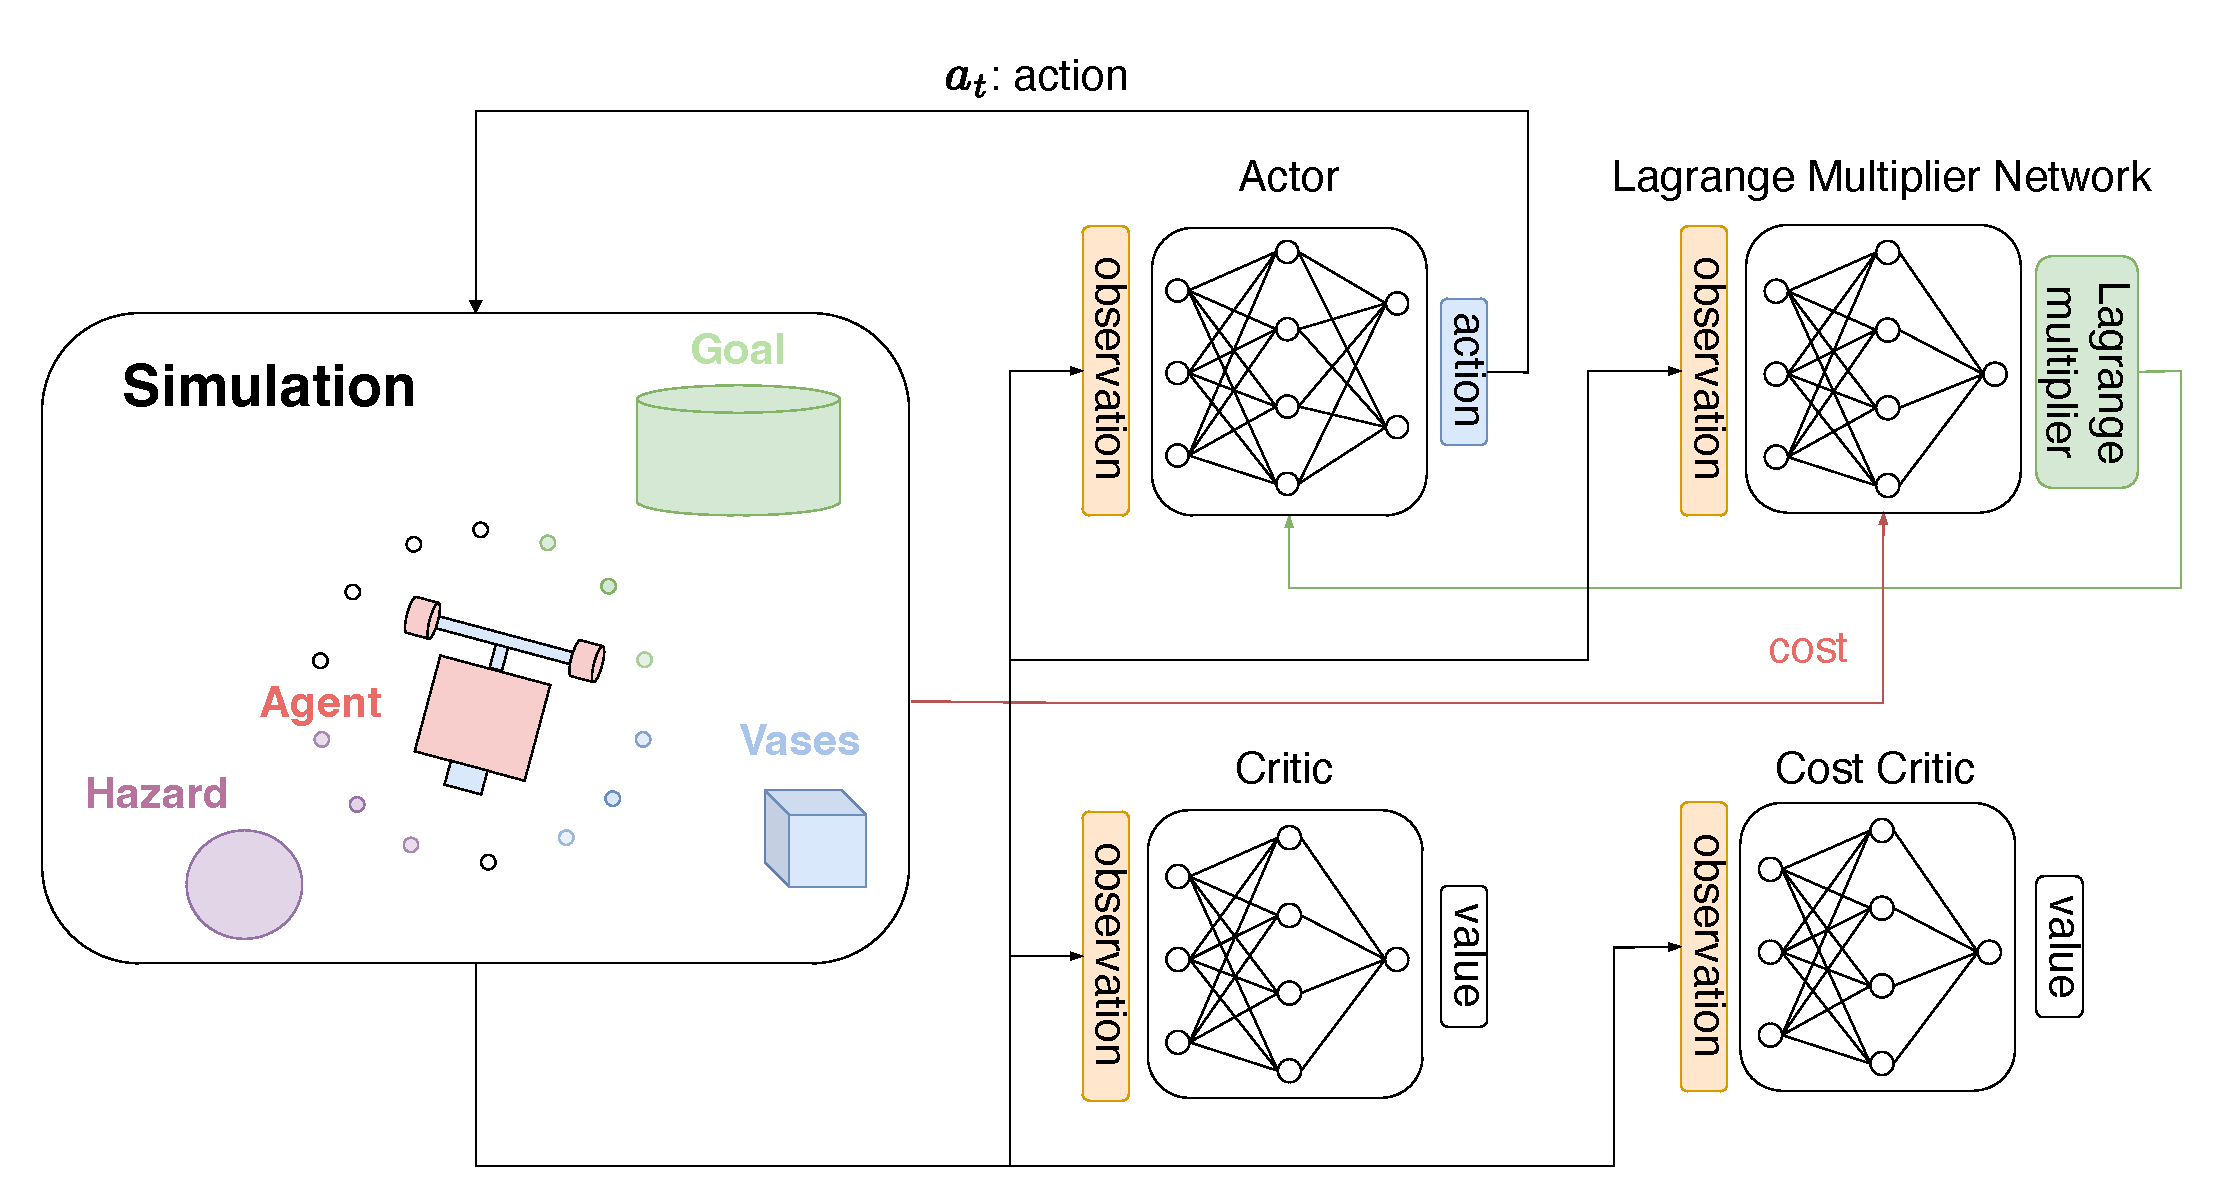
\includegraphics[width=0.8\linewidth]{figure/ppo_lagnet.pdf}
    \caption{Overview of the proposed method.
            Unlike standard PPO-Lagrangian, which employs a scalar Lagrange multiplier \textcolor{red}{since} the constraint is defined on cumulative cost, our approach imposes constraints in a state-wise manner, requiring state-varying multipliers. 
            To estimate these multipliers, we introduce an additional neural network, termed the Lagrange multiplier network.}
    \label{fig:ppo_lagnet}
\end{figure}

% TODO: PPO Lagrangian에 대한 설명이 없음
% TODO: PPO Lagrangian과의 차이를 명확히 언급 (단순히 NN을 썼다고 한 것만으로는 불충분)
In this paper, we propose a method that extends PPO Lagrangian to the state-wise constrained RL setting by estimating state-wise Lagrange multipliers.
Similar to PPO Lagrangian in Eq.~\eqref{eq:ppo_lagrangian_objective}, which employs a scalar Lagrange multiplier to handle constraints on the cumulative cost, addressing the state-wise constraint defined in Eq.~\eqref{eq:statewise_cost_return} requires a state-varying multiplier.
To this end, we introduce an additional neural network, referred to as the Lagrange multiplier network, which maps \textcolor{red}{each} state to its corresponding Lagrange multiplier, as illustrated in Fig.~\ref{fig:ppo_lagnet}.
Formally, the Lagrange multiplier network is parameterized by $\xi$ and is denoted as $\lambda_\xi(s)$.
This enables the application of Lagrangian relaxation to the constrained policy optimization defined in Eq.~\eqref{eq:scmdp_optimization_problem}, analogous to the way PPO-Lagrangian handles cumulative cost constraints.
The objective function of the proposed method can thus be expressed as:
\begin{equation} 
    \begin{aligned} J^{\text{Proposed}}(\theta) 
        = \mathbb{E}_{\pi_{\theta_\text{old}}} \Big[ &\min \big( r(\theta) A^{\pi_{\theta_\text{old}}}(s, a), \text{clip}(r(\theta), 1 - \epsilon, 1 + \epsilon) A^{\pi_{\theta_\text{old}}}(s, a) \big) 
        \\ &- \lambda_\xi(s) r(\theta) A^{\pi_{\theta_\text{old}}}_c \Big] 
    \end{aligned} 
\end{equation}
The parameters of the Lagrange multiplier network are updated using the following objective:
\begin{equation} \label{eq:lagrange_multiplier_update}
    J_\lambda(\xi) = \mathbb{E}_{(s_t, a_t, s_{t + 1}) \sim \tau, \tau \sim \pi_{\theta_\text{old}}} [\lambda_\xi(s_t) (C(s_t, a_t, s_{t + 1}) - w)]
\end{equation}
where $w$ denotes the state-wise cost limit.  % ! 여기서도 w로 표기했는데, 이럴 경우 설명의 편의를 위해 constraint가 하나라고 언급하는 방향으로 수정하는게 좋을듯?
In this formulation, the objective $J_\lambda(\xi)$ \textcolor{red}{encourages} the multiplier $\lambda_\xi(s)$ to increase when the observed cost $C(s_t, a_t, s_{t+1})$ exceeds the limit $w$, and to decrease when it falls below $w$.

\section{Experiments}

We evaluate our approach in the Safety Gymnasium \cite{ji2023safety} environment, \textcolor{red}{focusing on the \texttt{PointGoal} task under different cost limits.}
Safety Gymnasium provides two cost definitions: a binary indicator and object-specific values. 
We adopt the object-specific cost (\texttt{constrain\_indicator=False}) in all experiments.
We evaluate our approach in terms of constraint satisfaction performance by comparing it with CPO \cite{achiam2017constrained}, PPO Lagrangian \cite{ray2019benchmarking}, IPO \cite{liu2020ipo}, and CPPO \cite{stooke2020responsive}, using the implementations provided by Omnisafe \cite{ji2024omnisafe}.

\subsection{\textcolor{red}{Results}}

Figures.~\ref{fig:point_goal_results_vertical1} and \ref{fig:point_goal_results_vertical2} present the comparison on the \texttt{PointGoal} task under different cost limits.
Each figure shows how return, cost return, and the Lagrange multiplier evolve during training, highlighting how varying cost limits affect the agent's performance and constraint satisfaction.
Since all methods except ours define the constraint in terms of cumulative cost, \textcolor{red}{the threshold for our method was set to 1/1000 of theirs (as each episode consists of 1,000 steps).}
As shown in Fig.~\ref{fig:point_goal_results_vertical1} (b), (e), and Fig.~\ref{fig:point_goal_results_vertical2} (b), (e), our proposed method consistently satisfies the constraints across different constraint settings, unlike the other methods.
However, as the constraints are enforced more strictly, the reward performance is lower compared to some of the other methods, as shown in Fig.~\ref{fig:point_goal_results_vertical1} (d).
This is a common trade-off in constrained RL.
In addition, as shown in Fig.~\ref{fig:point_goal_results_vertical1} (f) and Fig.~\ref{fig:point_goal_results_vertical2} (c) and (f), when comparing the values of the Lagrange multiplier, our proposed method satisfies the constraints, resulting in bounded values or even decreasing trends.
An exception occurs when the cost limit is set to 0.5, which is particularly strict and difficult to satisfy, leading to continuously increasing values.

\begin{figure}[H]
    \centering

    % ----- 공통 범례 -----
    \begin{subfigure}{0.65\textwidth}
        \centering
        
\includegraphics[width=\linewidth]{figure/PointGoal/limit 1/legend_common.pdf}
    \end{subfigure}

    \vspace{0.5em} % 범례와 밑 그림 사이 간격 조정

    % ----- Limit 0.5 (왼쪽 열) -----
    \begin{minipage}{0.48\textwidth}
        \centering
        \begin{subfigure}{\linewidth}
            \centering
            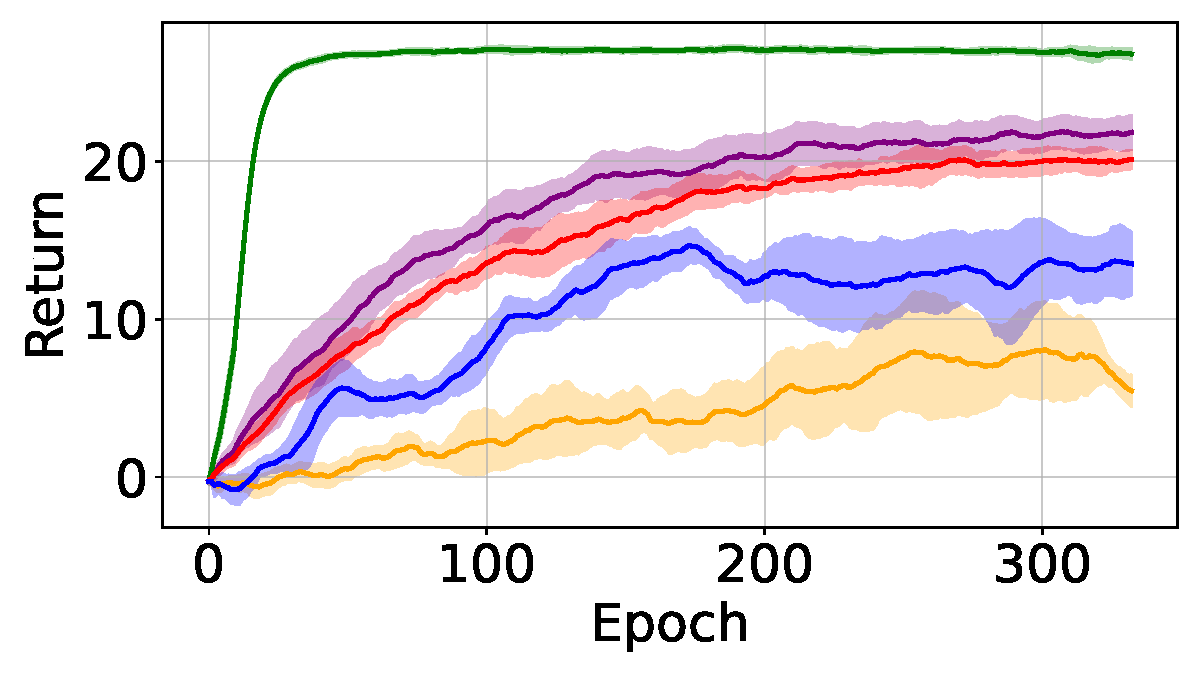
\includegraphics[width=\linewidth]{figure/PointGoal/limit 0.5/EpRet.pdf}
            \caption{Return over epochs}
        \end{subfigure}

        \begin{subfigure}{\linewidth}
            \centering
            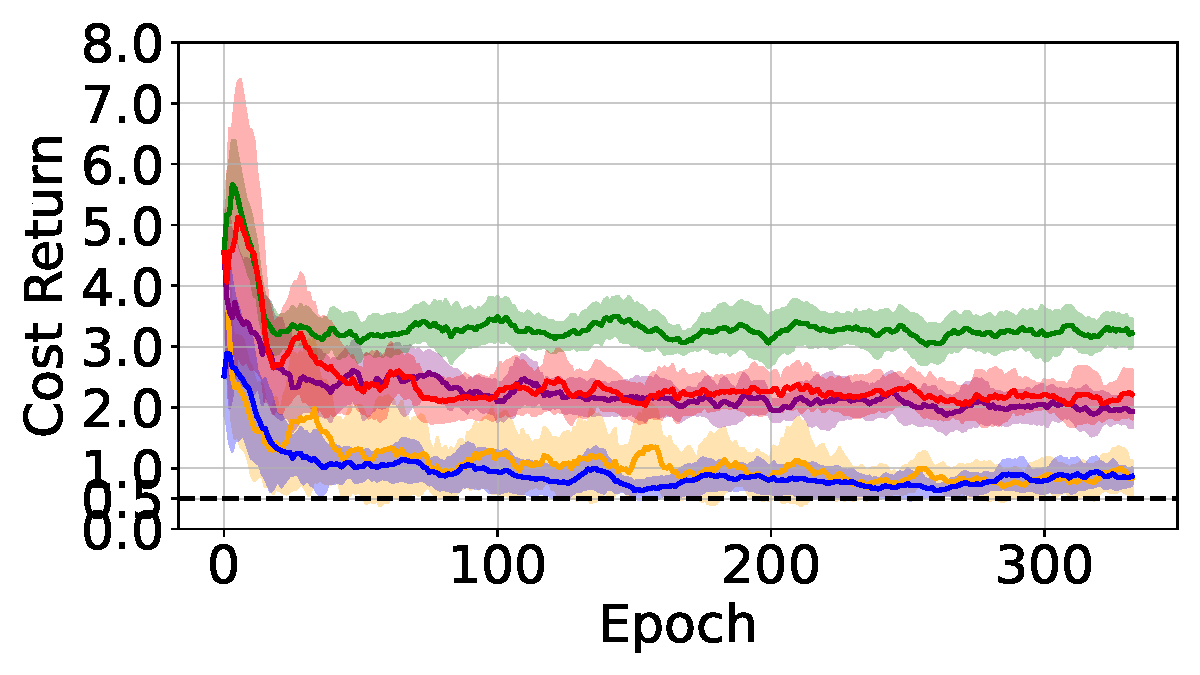
\includegraphics[width=\linewidth]{figure/PointGoal/limit 0.5/EpCost.pdf}
            \caption{Cost Return over epochs}
        \end{subfigure}

        \begin{subfigure}{\linewidth}
            \centering
            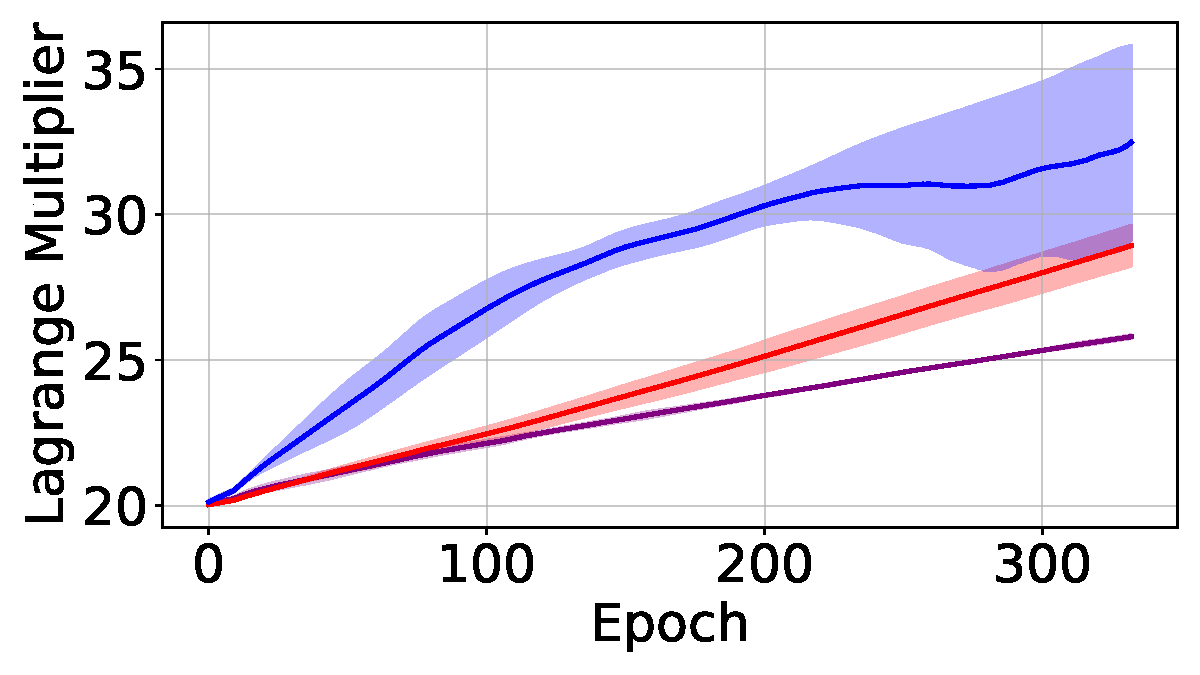
\includegraphics[width=\linewidth]{figure/PointGoal/limit 0.5/lagrange.pdf}
            \caption{Lagrange multipliers over epochs}
        \end{subfigure}

        \caption*{Cost return limit: 0.5}
    \end{minipage}
    \hfill
    % ----- Limit 1 (오른쪽 열) -----
    \begin{minipage}{0.48\textwidth}
        \centering
        \begin{subfigure}{\linewidth}
            \centering
            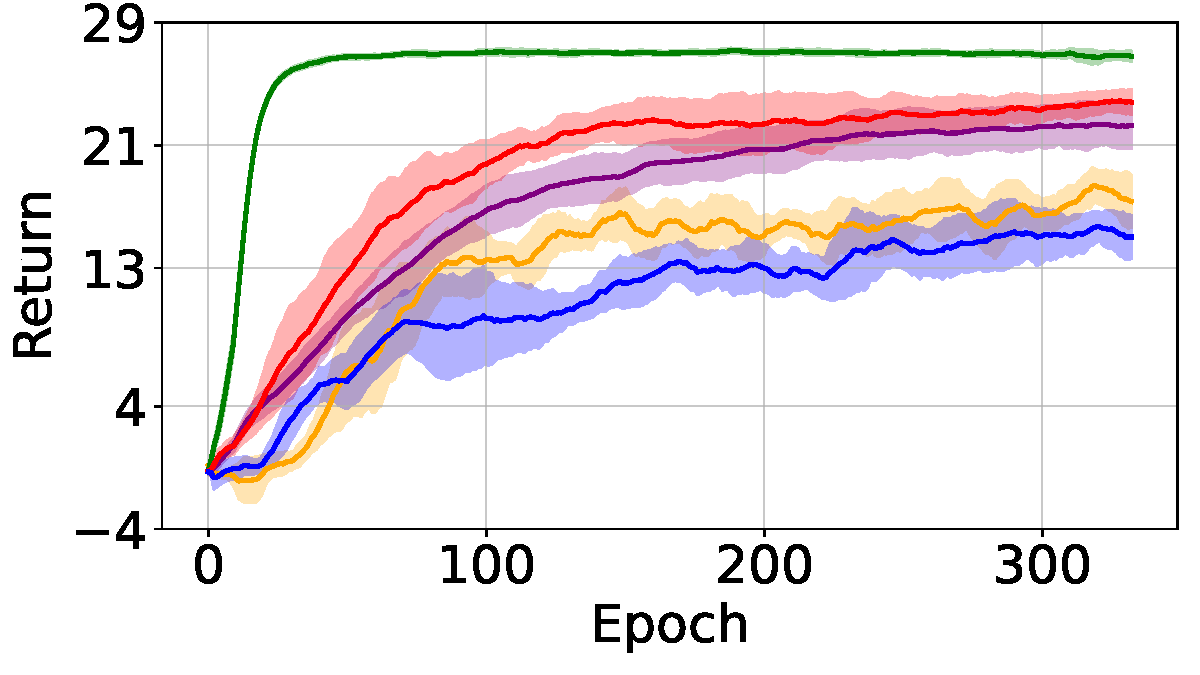
\includegraphics[width=\linewidth]{figure/PointGoal/limit 1/EpRet.pdf}
            \caption{Return over epochs}
        \end{subfigure}

        \begin{subfigure}{\linewidth}
            \centering
            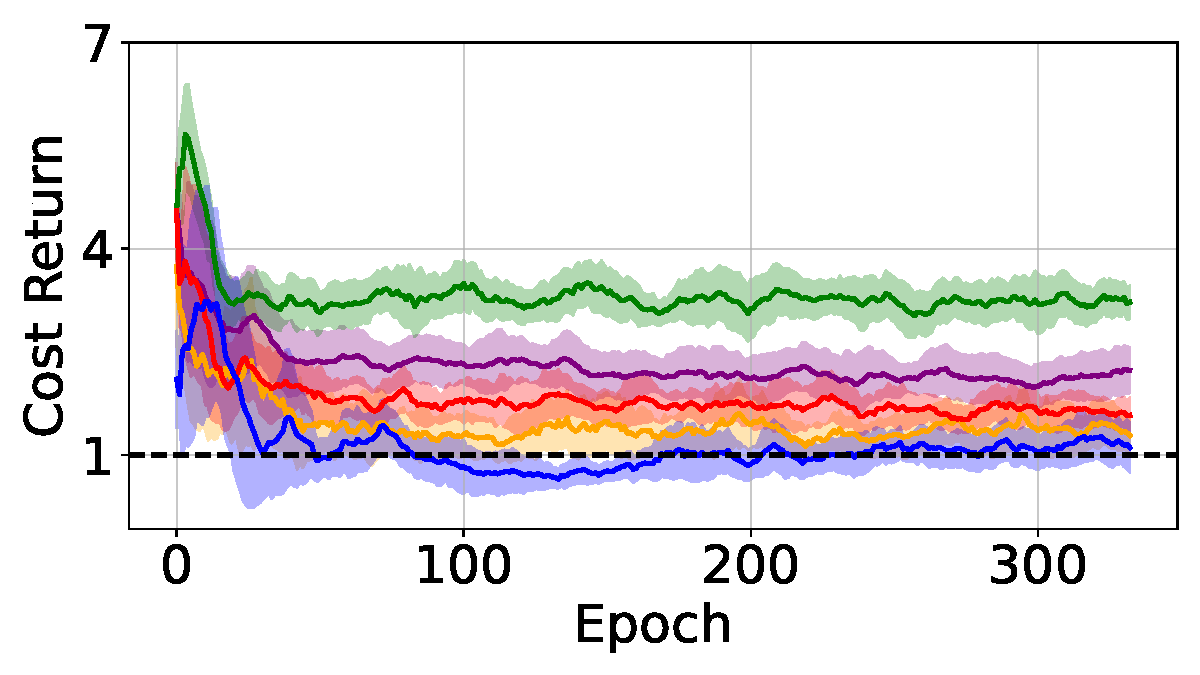
\includegraphics[width=\linewidth]{figure/PointGoal/limit 1/EpCost.pdf}
            \caption{Cost Return over epochs}
        \end{subfigure}

        \begin{subfigure}{\linewidth}
            \centering
            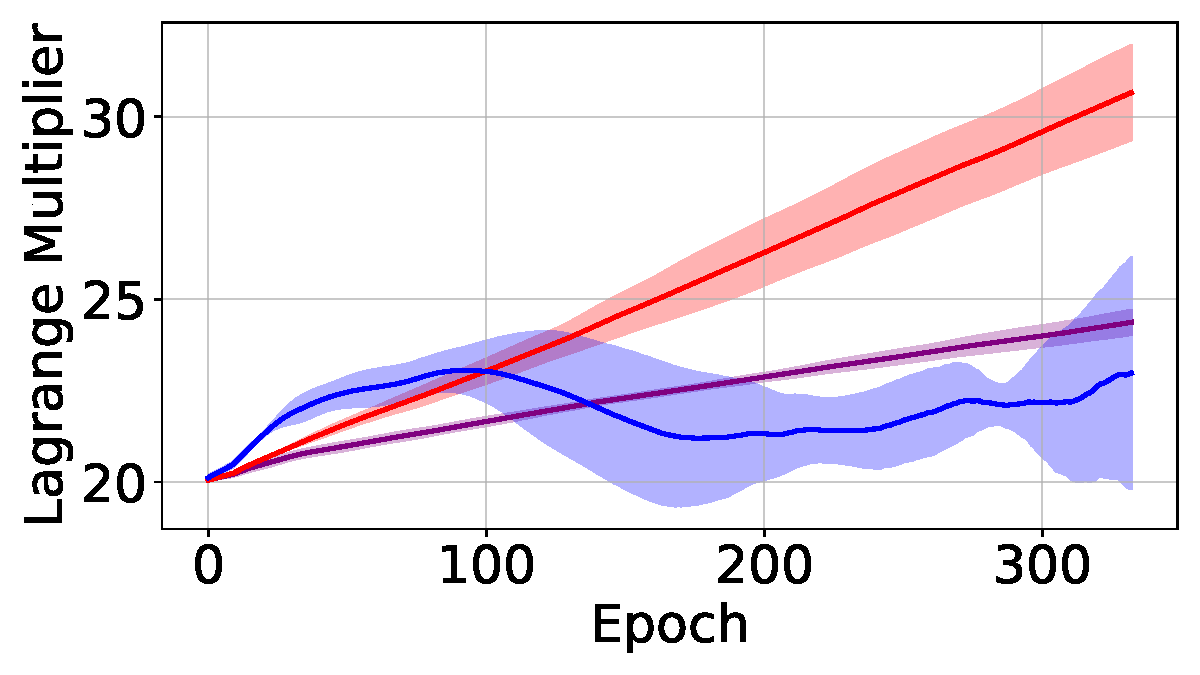
\includegraphics[width=\linewidth]{figure/PointGoal/limit 1/lagrange.pdf}
            \caption{Lagrange multipliers over epochs}
        \end{subfigure}

        \caption*{Cost return limit: 1}
    \end{minipage}

    \caption{\textcolor{red}{Learning curves.} 
    The left column, (a)–(c), illustrates the return, cost return, and Lagrange multiplier when the cost limit is set to 0.5. 
    The right column, (d)–(f), presents the corresponding results under a cost limit of 1.0. 
    Each row highlights a different metric, showing how the return (top), cost return (middle), and Lagrange multiplier (bottom) evolve over training epochs.}
    \label{fig:point_goal_results_vertical1}
\end{figure}

Here, the initial value of 20 was chosen empirically to accelerate convergence.
Unlike PPO Lagrangian and CPPO PID, which impose \textcolor{red}{constraints over cumulative costs across an episode} and therefore requires a single scalar multiplier, our method enforces state-wise constraints and thus needs \textcolor{red}{state-varying} multipliers.
\textcolor{red}{For our method, the state-wise multiplier values were averaged over each epoch for visualization.}

\begin{figure}[H]
    \centering

    % ----- 공통 범례 -----
    \begin{subfigure}{0.65\textwidth}
        \centering
        
\includegraphics[width=\linewidth]{figure/PointGoal/limit 2/legend_common.pdf}
    \end{subfigure}

    \vspace{0.5em} % 범례와 밑 그림 사이 간격 조정


    % ----- Limit 1.5 (왼쪽 열) -----
    \begin{minipage}{0.48\textwidth}
        \centering
        \begin{subfigure}{\linewidth}
            \centering
            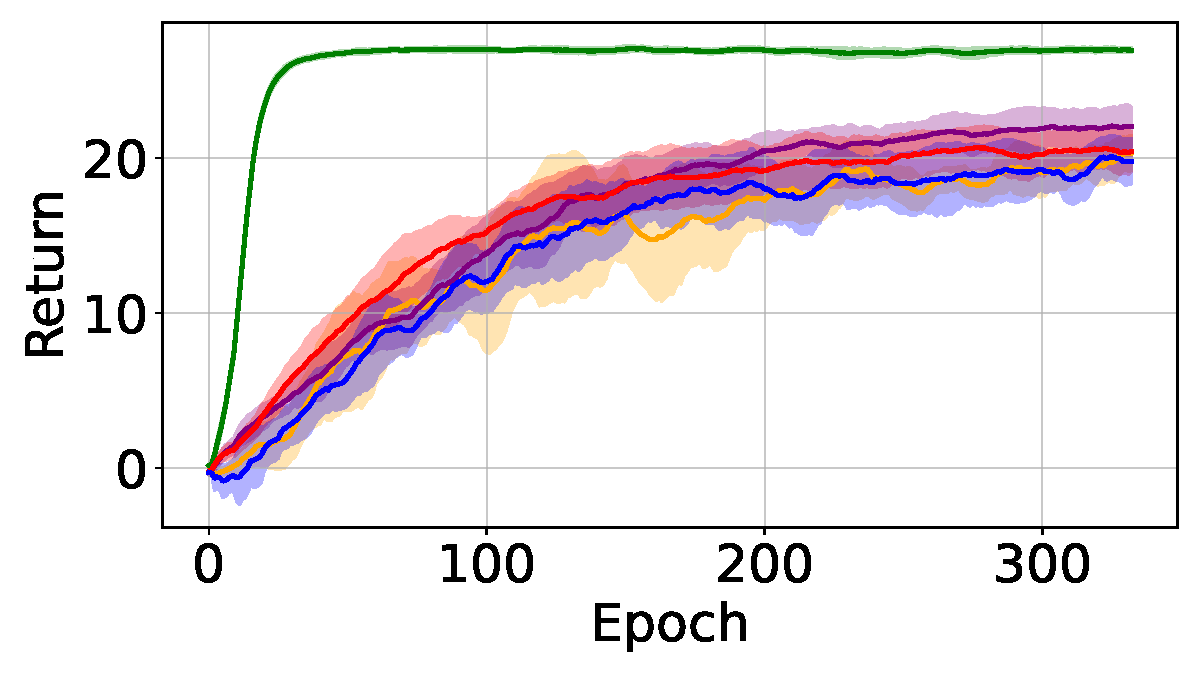
\includegraphics[width=\linewidth]{figure/PointGoal/limit 1.5/EpRet.pdf}
            \caption{Return over epochs}
        \end{subfigure}

        \begin{subfigure}{\linewidth}
            \centering
            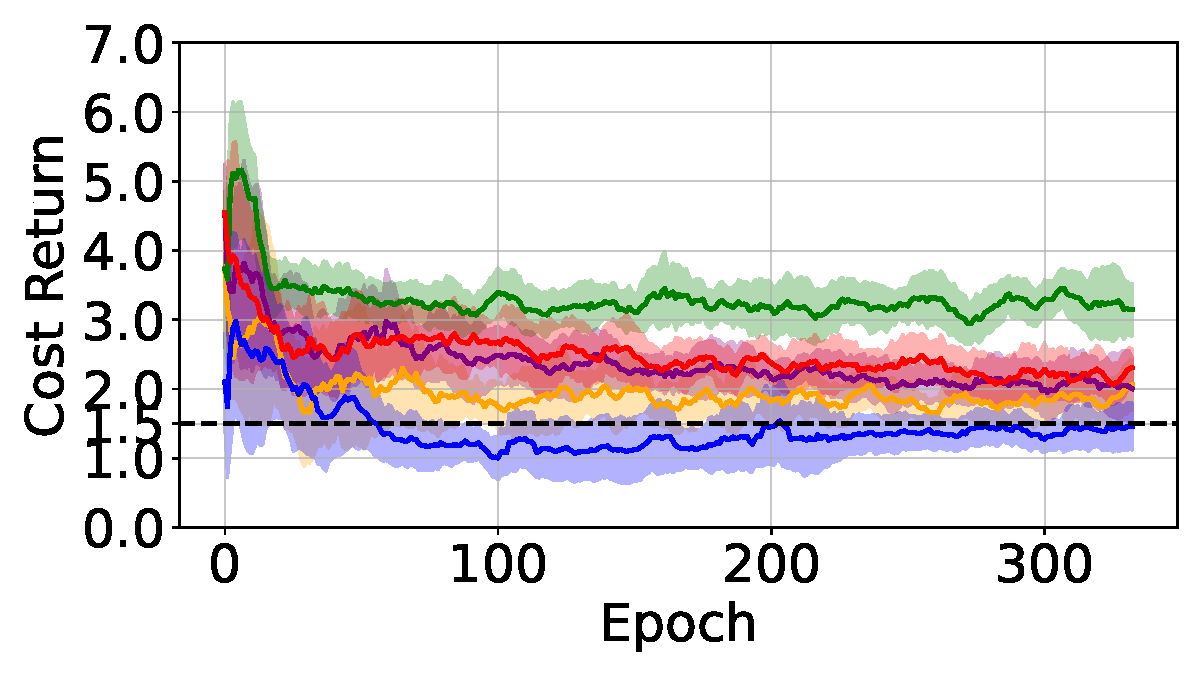
\includegraphics[width=\linewidth]{figure/PointGoal/limit 1.5/EpCost.pdf}
            \caption{Cost Return over epochs}
        \end{subfigure}

        \begin{subfigure}{\linewidth}
            \centering
            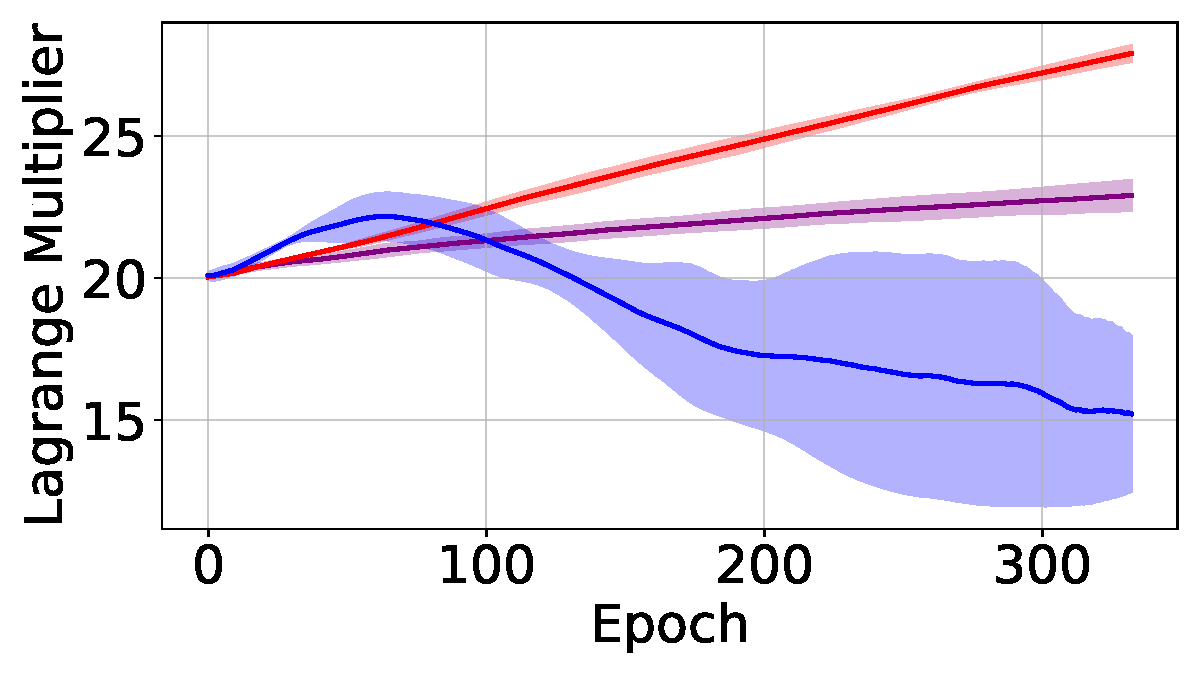
\includegraphics[width=\linewidth]{figure/PointGoal/limit 1.5/lagrange.pdf}
            \caption{Lagrange multipliers over epochs}
        \end{subfigure}

        \caption*{Cost return limit: 1.5}
    \end{minipage}
    \hfill
    % ----- Limit 2 (오른쪽 열) -----
    \begin{minipage}{0.48\textwidth}
        \centering
        \begin{subfigure}{\linewidth}
            \centering
            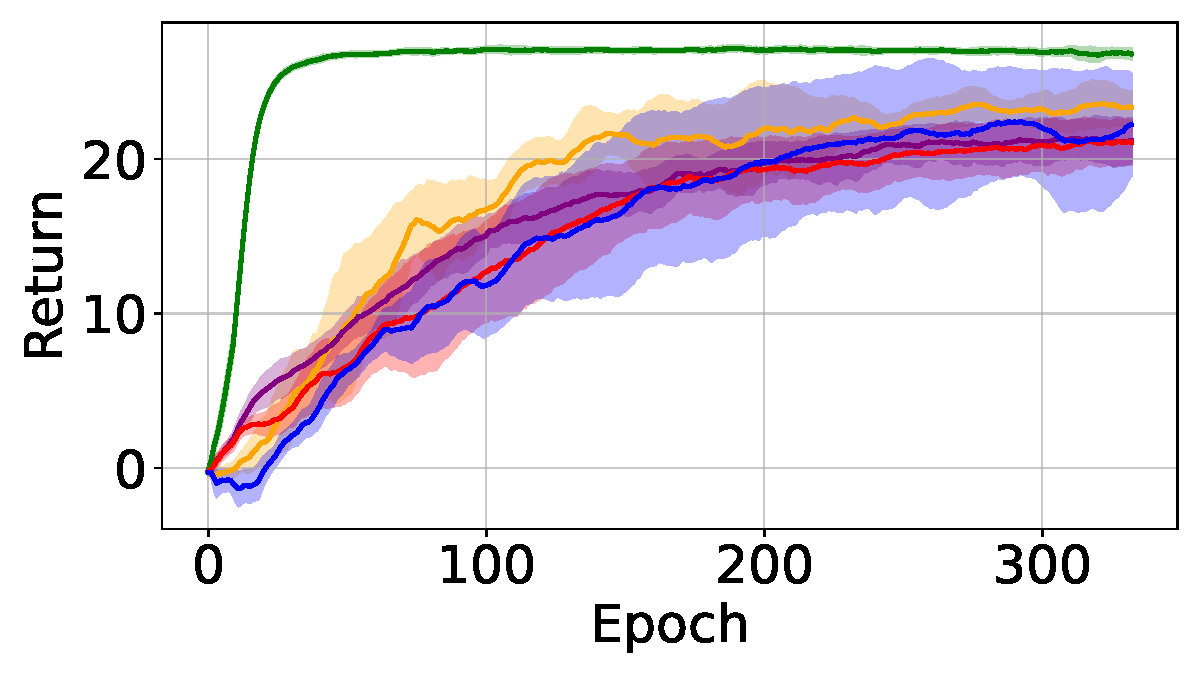
\includegraphics[width=\linewidth]{figure/PointGoal/limit 2/EpRet.pdf}
            \caption{Return over epochs}
        \end{subfigure}

        \begin{subfigure}{\linewidth}
            \centering
            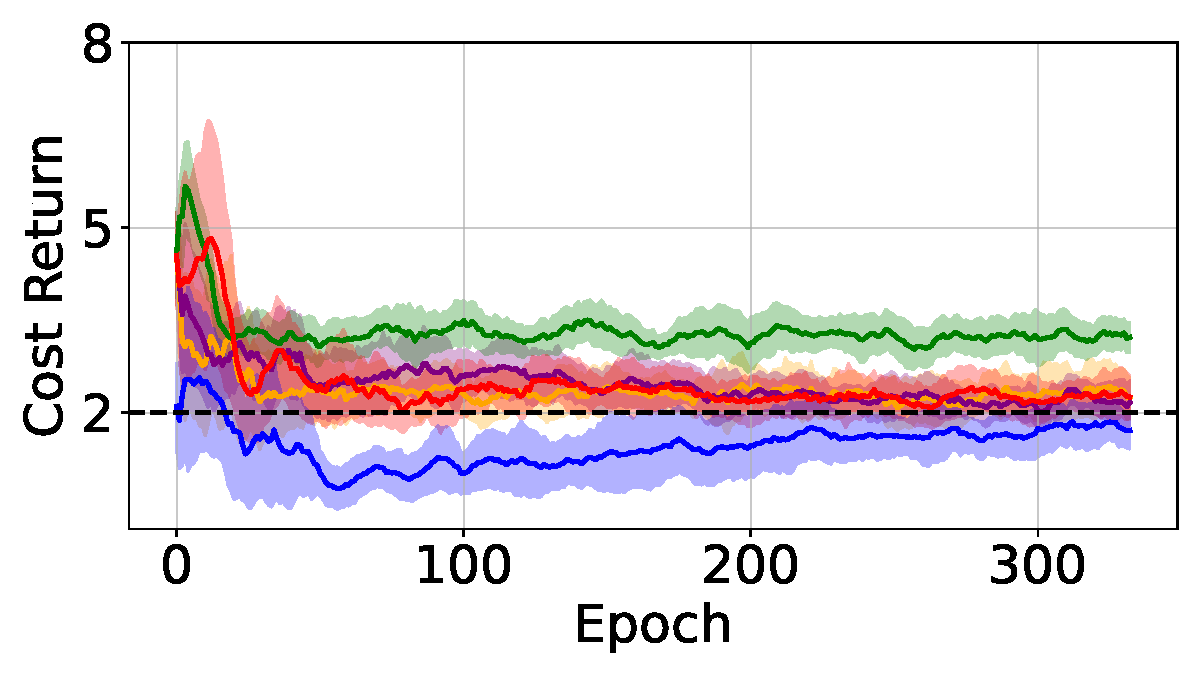
\includegraphics[width=\linewidth]{figure/PointGoal/limit 2/EpCost.pdf}
            \caption{Cost Return over epochs}
        \end{subfigure}

        \begin{subfigure}{\linewidth}
            \centering
            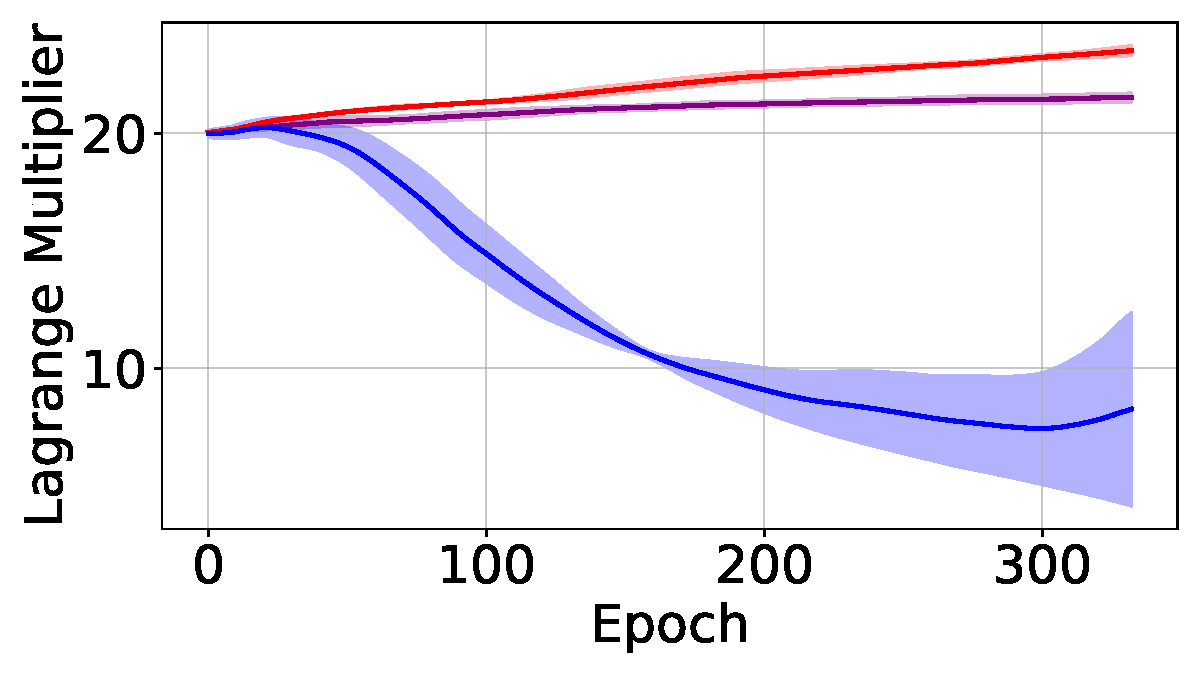
\includegraphics[width=\linewidth]{figure/PointGoal/limit 2/lagrange.pdf}
            \caption{Lagrange multipliers over epochs}
        \end{subfigure}

        \caption*{Cost return limit: 2}
    \end{minipage}

    \caption{\textcolor{red}{Learning curves.} 
            The left column, (a)–(c), illustrates the return, cost return, and Lagrange multiplier when the cost limit is set to 1.5. 
            The right column, (d)–(f), presents the corresponding results under a cost limit of 2.0. 
            Each row highlights a different metric, showing how the return (top), cost return (middle), and Lagrange multiplier (bottom) evolve over training epochs.}
    \label{fig:point_goal_results_vertical2}
\end{figure}

\subsection{\textcolor{red}{Analysis on Lagrange Multiplier}}

\textcolor{red}{Figures}~\ref{fig:point_goal_test_results_a} and \ref{fig:point_goal_test_results_bc} present the evaluation results of the learned Lagrange multiplier network. 
Figure~\ref{fig:point_goal_test_results_a} shows the per-step reward, cost, and the output of the network throughout a single episode. 
The output of the Lagrange multiplier increases as the agent approaches obstacles and potential constraint violations, while decreasing toward zero when the agent remains in safe states, as observed from the green curve in the bottom subplot of Fig.~\ref{fig:point_goal_test_results_a}.
Figure~\ref{fig:point_goal_test_results_bc} shows simulation frames corresponding to the two starred timesteps in Fig.~\ref{fig:point_goal_test_results_a}: the black star corresponds to subfigure (a), where the agent violates the constraint and the multiplier reaches its maximum value, while the white star corresponds to subfigure (b), where the agent remains in a safe state and the output stays close to zero.

% TODO: label 크기가 조금 작음. 별표도 작음.
% TODO: 별표 부분이 다음 figure에서 보여진다는 것도 언급
\begin{figure}[H]
    \centering
    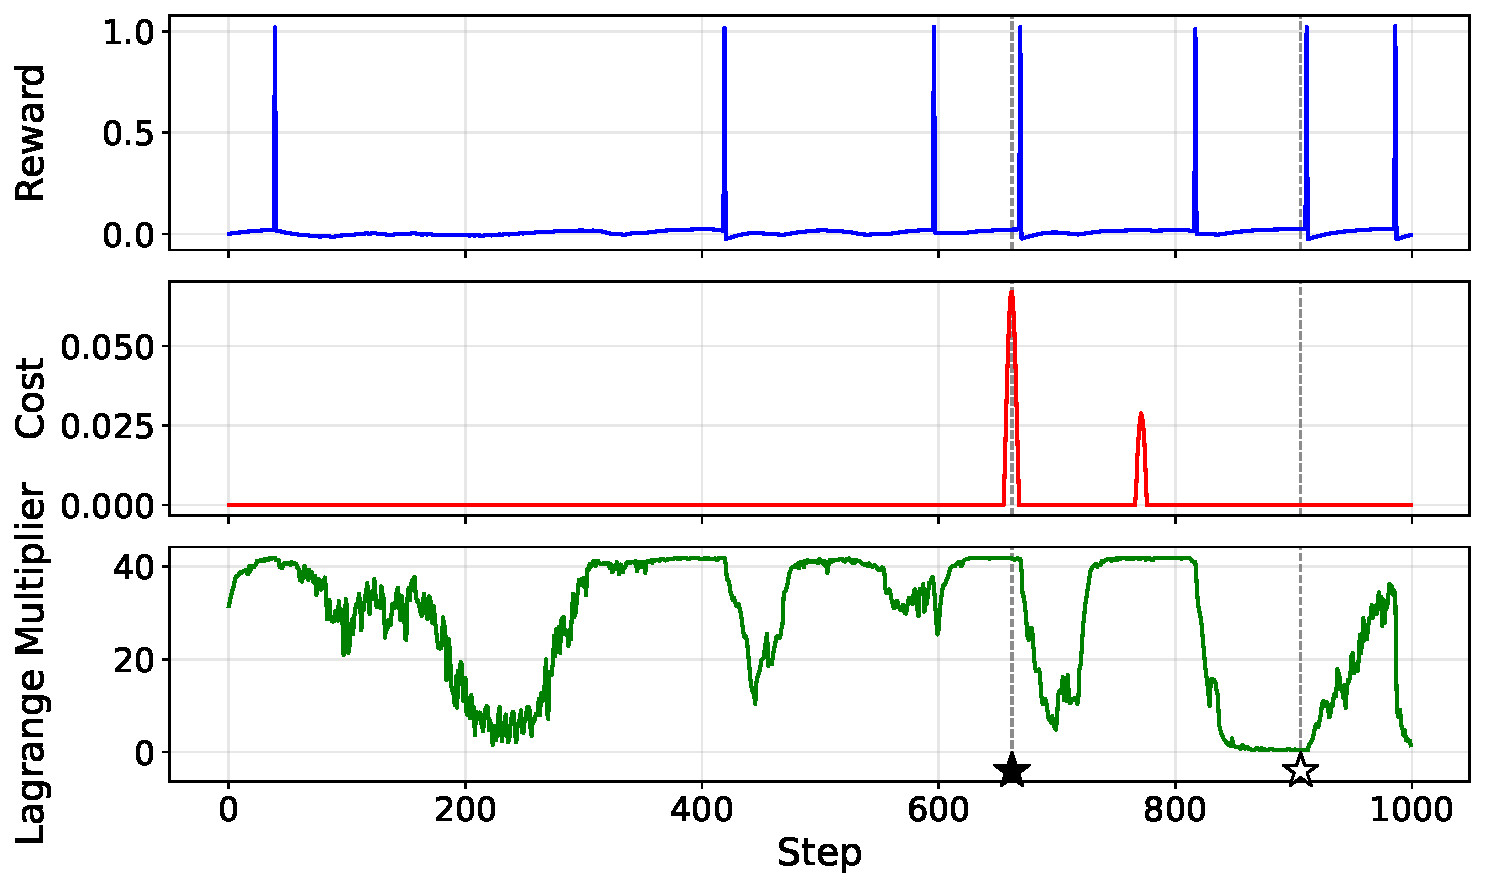
\includegraphics[width=0.8\textwidth]{figure/test/result.pdf}
    \caption{Evaluation results of a single episode. 
             The plot shows the per-step reward, cost, and the output of the learned Lagrange multiplier network. 
             The output increases as the agent approaches obstacles and constraint violations, while it decreases toward zero when the agent remains in safe states.}
    \label{fig:point_goal_test_results_a}
\end{figure}

\begin{figure}[H]
    \centering
    \begin{subfigure}{0.48\textwidth}
        \centering
        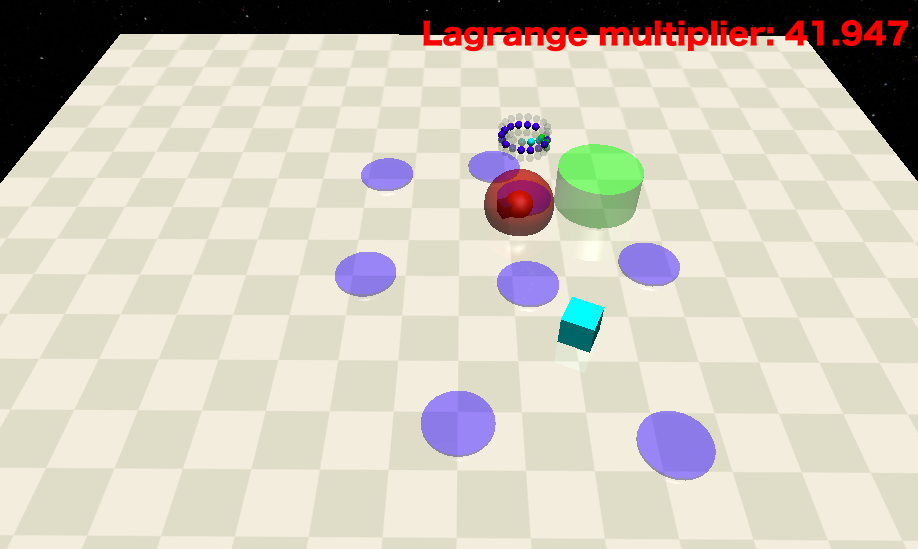
\includegraphics[width=\linewidth]{figure/test/unsafe.png}
        \caption{}
    \end{subfigure}
    \hfill
    \begin{subfigure}{0.49\textwidth}
        \centering
        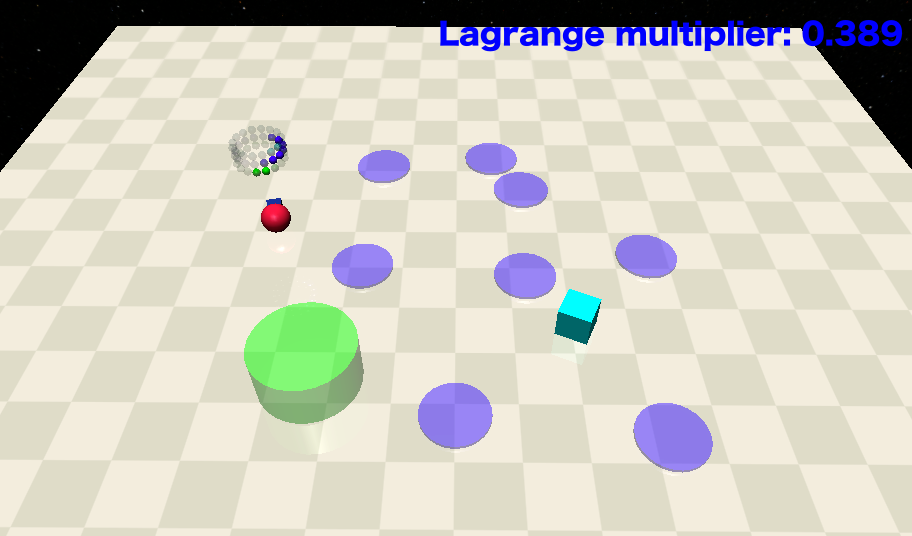
\includegraphics[width=\linewidth]{figure/test/safe.png}
        \caption{}
    \end{subfigure}
    \caption{Frames from the same episode at the timesteps marked with stars in Fig. ~\ref{fig:point_goal_test_results_a}. 
            Subfigure (a) shows the agent violating the constraint, where the network outputs its maximum value, 
            while subfigure (b) shows the agent in a safe situation, where the output remains close to zero.}
    \label{fig:point_goal_test_results_bc}
\end{figure}


\section{CONCLUSIONS}

In this work, we proposed a method that introduces state-wise Lagrange multipliers to learn policies that satisfy constraints defined \textcolor{red}{over} state-wise costs.
Unlike most existing approaches that address constraints based on cumulative costs, our method handles state-wise constraints, which inherently require state-dependent multipliers.
To this end, neural networks are employed to approximate these multipliers, enabling the policy to more effectively satisfy constraints at the level of individual states.
\textcolor{red}{The proposed approach allows for finer specification of constraints and demonstrates consistent satisfaction across experiments.}
Moreover, the learned Lagrange multiplier network can also be utilized at deployment to assess state-wise safety, thereby providing interpretability and insight into the agent’s behavior.

Building on \textcolor{red}{these} findings, future research could focus on two directions.
One \textcolor{red}{direction} is to pursue deterministic safety guarantees, for instance by leveraging the learned Lagrange multiplier network together with mechanisms such as safety filters or control barrier functions.
Another important direction is to improve sample efficiency, for example through off-policy or model-based approaches.

% This work demonstrates the potential of state-wise constrained RL and indicates that our approach could provide a promising foundation for developing safer and more interpretable RL agents.
\textcolor{red}{Overall, this work demonstrates the potential of state-wise constrained RL and suggests that our approach provides a promising foundation for developing safer and more interpretable RL agents.}
These contributions are expected to inspire further research on bridging theoretical safety guarantees and practical RL applications.
\begin{credits}
\subsubsection{\ackname}

This work was supported by the National Research Foundation of Korea (NRF) grant funded by the Korea government (MSIT) (RS-2025-00554087).

\subsubsection{\discintname}

\end{credits}

%
% ---- Bibliography ----
%
% BibTeX users should specify bibliography style 'splncs04'.
% References will then be sorted and formatted in the correct style.
%
\bibliographystyle{splncs04}
\bibliography{refs}
%

\end{document}
